\Chapter{Prezentáció példák}

% TODO: Tutorial jelleggel leírni, és bemutatni, hogy hogy lehet használni az alkalmazást.

A program jelenlegi verziójához nincs mellékelve grafikus felülettel ellátott projekt-szerkesztő, viszont a projekt sturktúra szabályait követve létrehozhatunk új prezentáció leíró állományokat.

\bigskip

\dirtree{%
.1 /presentation\_project01.
.2 /images.
.3 button.png.
.3 tuner.png.
.3 \ldots.
.2 /preferences.
.3 canvasses.json.
.3 settings.json.
.3 windows.json.
.2 scene.json.
.2 actions.py.
}

\bigskip

\noindent A projekt fájl \textit{JSON} állományokból, képekből és egy \texttt{actions.py} modulból áll, amelyben leírásokat adhatunk a \textit{Button} és a \textit{Tuner} widgetek viselkedésére.

A \texttt{/preferences} jegyzékben pedig általános beállításokra vonatkozó leírásokat adhatunk meg. A \texttt{settings.json}-ben a \textit{videófolyam}, a \textit{Rács} és a \textit{Hőtérkép} paramétereit adhatjuk meg. A
\texttt{canvasses.json}-ben pedig, ha igényt tartunk rá, a \textit{Vektormező} és a \textit{Globális eredővektor grafikon} vásznak tulajdoságait állíthatjuk be.
A \texttt{windows.json}-ben pedig az OpenCV által megjelenítendő ablakokat állíthatjuk be. A prezentációs során csak egy teljesképernyős ablakra van szükségünk, melyben a kimeneti képet láthatjuk. Ha csak az eredmény érdekel bennünket és nem tartunk igényt a program működésének megfigyelésére, akkor az utóbbi két fájl akár üresen is hagyható.

A \textit{DataParser} egység feldolgozza a felhasználó projekt fájlait és a bennük található leírások szerint futtatja a programot.

A \texttt{scene.json} állományban definiálhatjuk az egyes diák tartalmát. Az állomány egy lista, melynek elemei a \textit{JSON} objektummal leírt diák. A jelenlegi verzióban csupán egyetlen mezőt tartalmaznak a diákat leíró objektumok, a \texttt{widgets}-et. Ha később további információkkal szeretnénk ellátni a diákat (például metadatokat, egyéb leírásokat, további funkciókat szeretnénk jelölni), ezen a szinten tehetjük meg. A \texttt{widgets}-en belül pedig a widgetek listáját találjuk. Az egyes widget típusok különféle paraméterekkel rendelkeznek.\\
Példaként tekintsünk egy egyetlen diával rendelkező \texttt{scene.json} állományt, melyen egyetlen \textit{Tuner} widget helyezkedik el:
\begin{verbatim}
[
    {
        "widgets": [
            {
                "type":        "Tuner",
                "position":    [420, 300],
                "dimension":   [150, 150],
                "image":       "images/tuner.png",
                "min_value":   80,
                "max_value":   200,
                "transparent": true,
                "action":      "sample_action$arg"
            }
        ]
    }
]
\end{verbatim}
Jól látható, hogy a widgeteket \textit{JSON} objektumokként írhatjuk le, \texttt{type} mezőben jelöljük a widget típusát, az utána következő mezőkben pedig a widget paramétereinek értékeit adhatjuk meg. A \texttt{transparent} mezőben jelölhetjük, hogy kívánjuk-e használni a widget képének $\alpha$ csatornáját. Ha \texttt{true} értékkel látjuk el ezt a mezőt, akkor a program $\alpha$ csatornával eggyütt olvasssa be a képet, \texttt{false} esetén pedig csupán csak a három színcsatornára számít. Az $\alpha$ csatornával ellátott widget képek az $\alpha$ értékeiknek megfelelően rajzolódnak ki.
Az \texttt{action} mezőben pedig a widget-hez tartozó függvény nevét jelölhetjük, az \texttt{actions.py}-ból, illetve a \texttt{\$} szimbólum után egy további adatot is megadhatunk argumentumként, melyet stringként olvas be a \textit{Parser}. Ezt az adatot a futás során bármilyen formában felhasználhatjuk a widgethez tartozó függvényen belül.

A következőkben két példa prezentáción keresztül szeretném bemutatni a program lehetséges használati módjait. Az első példa prezentációban pár képfeldolgozó módszer kerül bemutatásra, a második pedig a dolgozatomról szól.
A videófolyamon megjelenő widget-ek képeit \textit{GIMP (GNU Image Manipulation Program)} képszerkesztő segítségével szerkesztettem meg. Az elkészült képek csupán szemléltetésre szolgálnak. Minőségi, szemetgyönyörködtető, alfa csatornával rendelkező widgetek használatával még látványosabbá tehetjük a prezentációnkat. Egy egységesített, felhasználóbarát widget szerkesztő megoldhatná a külső képszerkesztő használata során adódó kényelmetlenségeket. A szöveg helyét néhány helyen a \textit{Lorem ipsum} szövegrészlet vagy angol nyelvű szöveg tölti ki.

\Section{Képfeldolgozás, OpenCV bemutatása}

Az első példaprezentáció a képfeldolgozás témakör köré épül és bemutatásra kerül az \textit{OpenCV} is. A programom segítségével a témakört egy új megközelítésben ismertethetjük. Az egyes képfeldolgozó technikákat valós időben mutathatjuk be, a videófolyamot manipulálva, dinamikus paraméterezés mellett. Az így megvalósított prezentáció, látványosabb és kifejezőbb, szemléletesebb lehet a hagymányos prezentációs eszközökkel megvalósított előadásoknál.

Összeállításánal igyekeztem kihasználni a programom edddig elkészült állapotainak lehetőségeit. A widgetek paramétereit a fejezet bevezetésében leírtak alapján állítottam be a \texttt{scene.json} állományban. Az állomány tíz darab objektuma a tíz fóliát jelöli.\\
A diasor szerkezete a következő:
\begin{itemize}
	\item Bevezetés
	\item Menü
		\begin{itemize}
			\item Digitális képek
			\item \textit{Alpha Blending}
			\item Küszöbölés technika
			\item Éldetektálás
			\item Különböző filterek/szűrők bemutatása
				\begin{itemize}
					\item Gauss-elmosás
					\item Hisztogram kiegyenlítés
				\end{itemize}
		\end{itemize}
	\item Befejezés
\end{itemize}
Mint láthatjuk, a prezentációnak különböző szintjei vannak. A prezentációról egy képernyőképet \aref{fig:opencvdemo}. ábrán láthatjuk.

\begin{figure}[h]
\centering
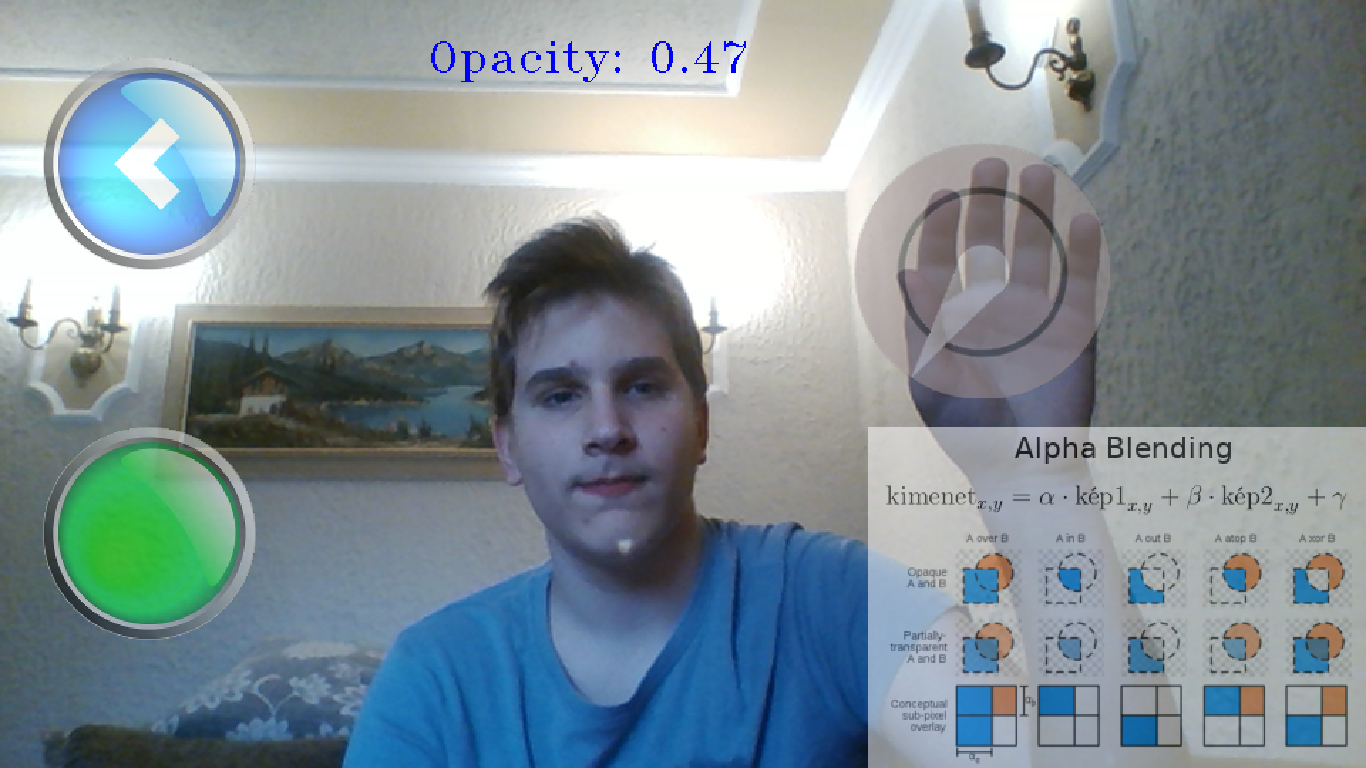
\includegraphics[width=\textwidth]{images/opencv_demo_screenshot.png}
\caption{Képernyőkép a demoról}
\label{fig:opencvdemo}
\end{figure}

Az első dián szereplő \textit{Rollable} widget tartalmazza a bevezetést, amely egy rövid áttekintés, hogy miről is fog szólni a prezentáció. Egy \textit{Shiftable} típusú \textit{OpenCV} logó is helyet kapott itt, illetve egy \textit{Button} típusú widget, melynek a funkciója a léptetés, melynek függvénye az \texttt{actions.py} modulon belül található meg. A prezentációban szereplő léptetést a \texttt{scene.json} állományban a következő módon jelölhetjük:
\begin{verbatim}
"action": "jump_to$1"
\end{verbatim}
Bárhol járjunk az előadásban, a fenti jelöléssel ellátott \textit{Button} az 1-es indexű fóliára fog eljuttatni minket. A \texttt{jump\_to} függvény pedig a következőképpen néz ki:
\begin{python}
def jump_to(controller, button_widget):
    if button_widget.pushed:
        controller.current_scene = int(button_widget.arg)
        button_widget.pushed = False
\end{python}
A függvény paramétereként átadódik a \texttt{controller} és a \texttt{button\_widget} címe, melyeket elérve módosíthatjuk a program aktuális állapotait. Ha ezen funkcióval ellátott \textit{Button} típusú gomb lenyomódik, akkor az éppen aktuális fólia sorszámát manipuláljuk az argumentumként kapott adattal, melyet \texttt{int} típusúvá, azaz egész számmá konvertálunk. A művelet végén a gomb lenyomását megszűntethetjük, így ha vissza kell lépnünk erre a fólira, nem okoz majd gondot a lenyomva maradt gomb, amely a fóliára lépés pillanatában újra elnavigálna a benne jelzet fóliára.
A példaprezentációra jellemző, hogy előre és hátra is léptethetjük a fóliákat, így bejárva az összes szintet.

A második fóliát egy menürendszernek szántam. A csempeszerűen elhelyezkedő widgetek segítségével érhetjuk el rajtuk jelölt funkciókat. A diavetítés így nem lineáris lesz, hiszen szabad sorrendben lefuttathatjuk azokat. Ezen widgetek \textit{Button} típusúak, a hozzájuk tartozó művelet pedig az aktuális diát jelző pointer értékének változtatása a cél helyre, vagyis a már említett \texttt{jump\_to} függvénnyel való ugrás. Ezen diák szintén a \texttt{scene.json} elemei, sorban, a Menü fólia után helyezkednek el.

Az Menüből elérhető diák tartalma változó, a hozzájuk tartozó témakör kifejtését tartalmazzák. A dinamikus elemekkel ellátott diákon a témakörnek megfelelően elhelyzetem olyan vezérlőket, melyekkel manipulálhatjuk a kimeneti videófolyamot a témakörök szemléletesebb bemutatása érdekében.
Például a Küszöbölés technikát bemutató dián a funkciót aktiváló \textit{Button} megnyomása esetén a videófolyamon a \textit{Tuner} értékeinek megfelelően végrehajtódik a küszöbölés művelete. A \textit{Tuner} segítségével állíthatjuk a küszöb alsó határát, az eljárás szemléltetése érdekében.
Az éldetektálással és \textit{Alpha Blending} technikákkal foglalkozó fóliákon szintén hasonlóan demonstrálhatjuk a technikák működését, \textit{Tuner} widget segítségével értékeket állítva.
A filtereket bemutató fólia szintén egy menürendszer, melyen két \textit{Button} segítségével érhetejük el a kívánt fóliákat. A Gauss-elmosást és a hisztogram kiegyenlítést bemutató fóliákon található egy-egy \textit{Button} widget is, melynek megnyomása esetén a hozzátartozó művelet végrehajtódik. Például a Gauss-elmosással foglalkozó fólia ilyen \textit{Button}-ja a következő egyszerű függvénnyel rendelkezhet:
\begin{python}
def gauss_button(controller, button_widget):
    if button_widget.pushed:
        controller._video.frame = \
        		cv2.GaussianBlur(controller._video.frame,
					(19, 19),
					cv2.BORDER_DEFAULT)
\end{python}
A videófolyam aktuális képkockáját felülírjuk a \texttt{cv2.GaussianBlur()} kimenetével. Mivel a projektben definiált függvények lekezelése a feldolgozási folyamatok után történnek meg, így az ilyen módon módosított képkocka ezután csupán már csak megjelenítésre vár.

A módszereket bemutató diák mindegyikén elhelyezkedik egy-egy \textit{Button} típusú widget is, amellyel az eggyel korábbi szintre, vagy a Menübe léphetünk vissza.

A Menüből pedig szintén egy \textit{Button} segítségével léphetünk tovább az utolsó diára, ahol egy \textit{Expandable} widget segítségével foglalhatjuk össze a prezentációnkat és köszönhetjük meg a figyelmet.

\Section{Dolgozat bemutatása}

A második példaprezentáció segítségével a dolgozatomat szeretném bemutatni.
A prezentáció során a videófolyam az általános widgetek mellett valós időben frissülő ábrákkal is kiegészül, melyeket egyébként a program fejlesztői módú futása során láthatnánk. Ilyenek a \textit{Frame Difference}, \textit{Grab}, \textit{Vektormező} ábrák. A folyton frissülő ábrák segítségével a dolgozat kulcs elemeit szemléletesebben bemutathatjuk.

A prezentációban a dolgozatomban tárgyalt főbb elemek kerülnek említésre. A fejezetek szerint haladva kerül bemutatásra a témakör és a dolgozat anyaga. Egyedül a widgetek nincsenek külön bemutatva, hiszen azok a prezentáció teljes egészében jelen vannak. Az egyes fóliák közti léptetés az előző prezentációhoz hasonlóan van megoldva. A widgetek \textit{design}-ja is hasonló, viszont ennél a prezentációnál mellőztem a \textit{Lorem ipsum} és angol nyelvű szövegeket a tartalomelemeknél és törekedtem az informatív leírásokkal és szemléletes képekkel színesíteni a widgeteket.

Az első példaprezentációban használt menürendszeres megoldást itt is szeretném alkalmazni a prezentációk megszokott linearitását megtörve. Természetesen a prezentáció ajánlott menete így is lineáris marad, ez a fajta öszzeállítása az előadásnak csupán azért szükséges, hogy a logikailag egybefüggő részek még jobban elkülönüljenek egymástól. A fő fóliákból további alfóliák érhetők el. Nem célom labirintusszerűen felépíteni az előadást, hogy a prezentáló személy se tudjon kiigazodni a saját előadásában, így a lehetséges mélységi szintet minimalizálni fogom.\\
A prezentáció szerkezete a következő:
\begin{itemize}
	\item Bevezetés
	\item Koncepció
		\begin{itemize}
			\item Kiterjesztett valóság
			\item Prezentációs szoftverek
			\item \textit{OpenCV} és \textit{scikit-learn}
		\end{itemize}
	\item Gesztusok
		\begin{itemize}
			\item Optical-Flow
			\item \textit{Grid}/vektormező
				\begin{itemize}
					\item \textit{Sweep}
					\item \textit{Rotation}
					\item \textit{Shift}
				\end{itemize}
			\item \textit{Hőtérkép}
				\begin{itemize}
					\item \textit{Blink}
					\item \textit{Symbol}
				\end{itemize}
			\item Gépi tanulás
		\end{itemize}
	\item Példa prezentációk
	\item Összegzés, befejezés
\end{itemize}
Mint látható, különböző szinteket különíthetünk el. Az egyes szintek gyökéreleméhez egyetlen lépéssel vissza tudunk lépni, viszont a fóliákból a velük egy szinten lévő további fóliákat nem érjük el közvetlenül. Kivételt képeznek ez alól a legfelső szinten elhelyezkedő diasorok, közöttük szabadon lépkedhetünk.

A Bevezetés fóliában egy általános bevezetés megtételére van lehetőségünk. Említésre kerülhet a dolgozat feladata, melyet a későbbiekben részletesebben is ismertethetünk. Hasonlóan az első prezentációhoz, itt is egy \textit{Rollable} widgeten helyezkedik el a bevezetés tartalma.

\begin{figure}[h]
\centering
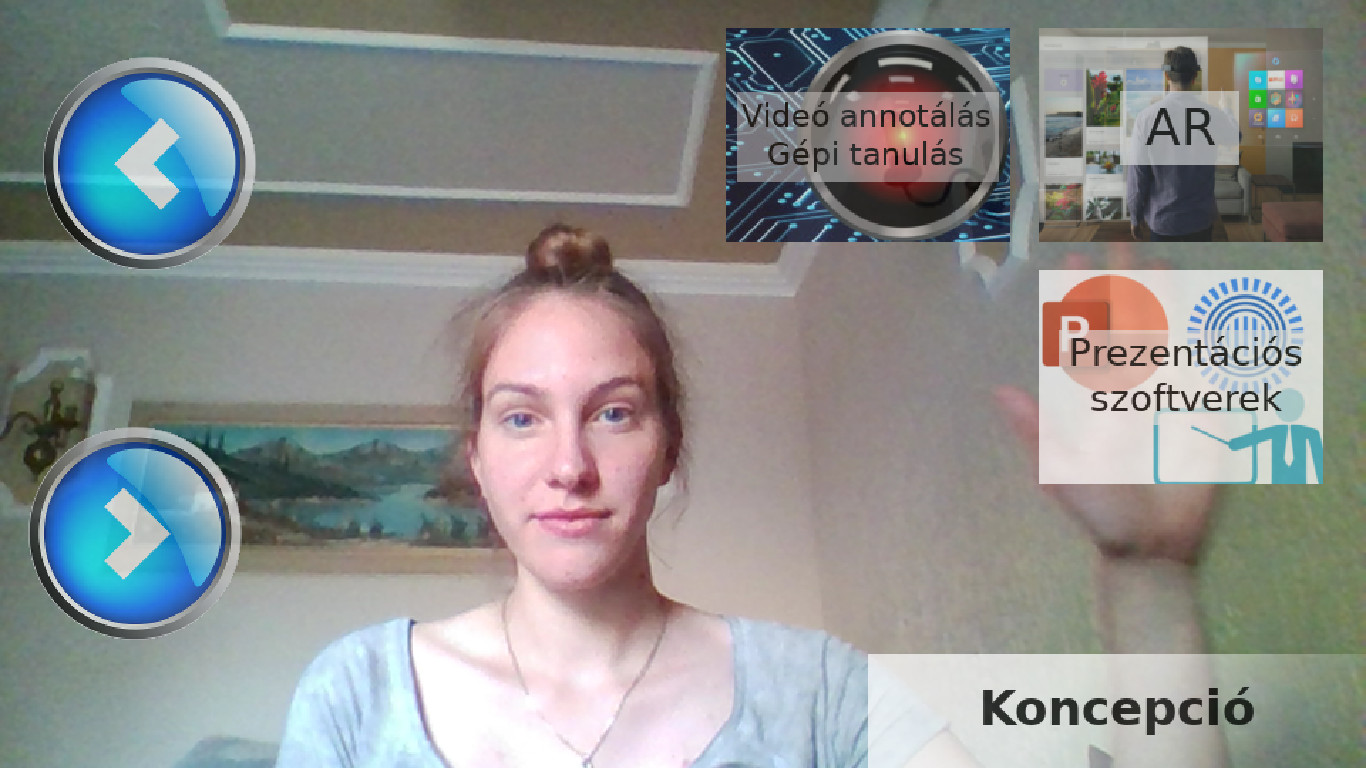
\includegraphics[width=\textwidth]{images/dolgozat_demo_screenshot.png}
\caption{Képernyőkép a demoról}
\label{fig:dolgozatdemo}
\end{figure}

A bal alsó sarokban elhelyezkedő \textit{Button} segítségével érhetjük el a következő diát, a Koncepció menüjét (\ref{fig:dolgozatdemo}. ábra), amelyről további fóliákat érhetünk el. Itt taláható meg a kiterjesztett valóság, prezentációs szoftverek, \textit{OpenCV} és \textit{scikit-learn}-el foglalkozó diasorok. Az itt szereplő widgetek még nem tartalmaznak élő-ábrákat, az általános widgetek segítségével mutthatjuk be az adott témaköröket. Ezen szekció célja az említett fogalmak tisztázása, általános bemutatása.

A Gesztusok fólia szintén egy menürendszert tartalmaz. Innen 4 további fóliát érhetünk el.
Itt találjuk meg az \textit{Optical-Flow}, a \textit{Grid}, a \textit{Hőtérkép} és a \textit{Gépi tanulás} diasorokat. A \textit{Grid} és \textit{Hőtérkép} fóliákkal egy újabb szintet érhetünk el. A hozzájuk kapcsolódó témaköröket belőlük tudjuk elérni. Itt már megjelennek a frissülő ábrák is, melyek segítségével szemléltesebben be tudjuk mutatni az adott témát.
A \texttt{scene.json} állományban a gomb argumentumaként megadott "default" kulcsszó segítségével a gombokon belüli funkció gombnyomás nélkül is elérhető lesz. Ezen apró trükk segítségével a diára lépés pillanatában megjelennek az élő ábrák. A "default" kulcs megléte az \texttt{actions.py} modulon belül található függvényekben kerül ellenőrzésre. Ez csupán csak egy példa az argumentum használatra. Amennyiben elmarad a kulcsszó a leíró állományban, a widget a gombnyomás után kezdi el frissíteni a saját képét a kívánt ábrára.

A példaprezentációkat tartalmazó fólia csupán csak említés szinten foglalkozik a példákkal. Az első példa widgetje \textit{Widget} típusú, vagyis semmilyen tulajdonsággal nem rendelkezik, csupán egy képet tudunk megjeleníteni a segítségével. A Dolgozattal foglalkozó példaprezentáció widget-je pedig egy \textit{Button}, melyet megnyomva visszatérhetünk a prezentáció legelső diájára.

A második példaprezentáció is hasonlóan ér véget, mint az első, egy \textit{Expandable} widget segítségével foglalhajuk össze az előadást és köszönhetjük meg a figyelmet.
